\subsection{Time Imaging Reconstruction}
\label{sec:ti}

The time-based imaging method is based on the approach used by the Belle II time-of-propagation (TOP) counter~\cite{staric2}. The basic concept is that the measured arrival time of Cherenkov photons in each single event is compared to the expected photon arrival time for every pixel and for every particle hypothesis, yielding the PID likelihoods.

The expected photon arrival time, which accounts for the time of flight of particle from interaction region to the fused silica radiator and for the propagation time of the Cherenkov photon produced by that particle in the radiator, can be calculated in different ways:
\begin{itemize}
\item The expected timing spectra can be calculated analytically based on the charged particle direction and hit location on the DIRC wall, as desctibed in~\cite{staric2, staric3}.
\item The full detector simulation can be used to produce timing spectra for each photon. Since the DIRC signal depends on the particle momentum, direction, and the position on the DIRC wall, the simulation of timing spectra for all charged particle configurations might be not feasible.
\item In beam tests, when the external PID is available, the timing spectra can be extracted from the data.
\end{itemize}

The second approach was used to evaluate the time-based imaging method for \gluex DIRC.

\begin{figure}[!h]
\centering
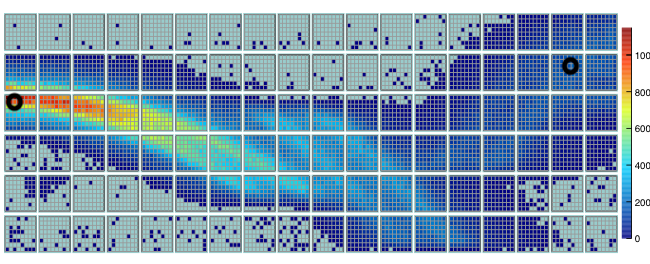
\includegraphics[clip, trim=0cm 0cm 0.5cm 0.1cm, width=0.58\textwidth]{pics/kaonsTI.png} \hspace{0.05\textwidth} 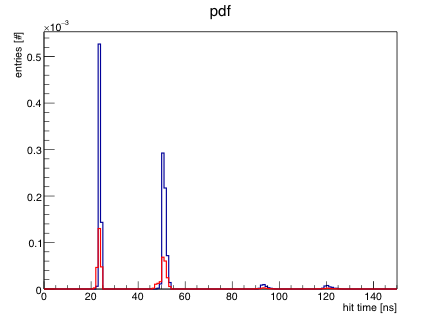
\includegraphics[clip, trim=0.75cm 0.35cm 0.35cm 0.52cm,width=0.35\textwidth]{pics/LeftPix.png}
\put(-140.,-8.){\small{photon propagation time [ns]}} \put(-70., 70.){\textcolor{red}{pions}} \put(-70., 50.){\textcolor{blue}{kaons}}  \\
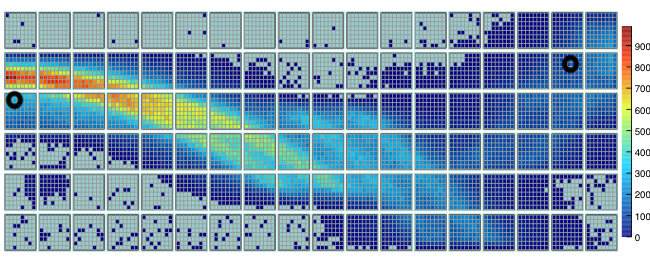
\includegraphics[clip, trim=0cm 0cm 0.5cm 0.1cm, width=0.58\textwidth]{pics/pionsTI.png} \hspace{0.05\textwidth} 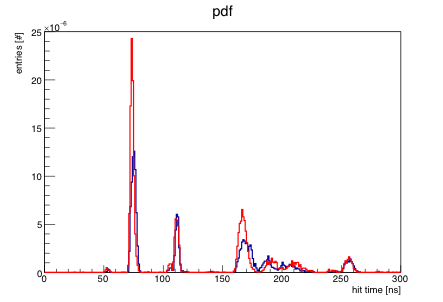
\includegraphics[clip, trim=0.75cm 0.35cm 0.35cm 0.52cm,width=0.35\textwidth]{pics/rightPix.png} 
\put(-140.,-8.){\small{photon propagation time [ns]}} \put(-70., 70.){\textcolor{red}{pions}} \put(-70., 50.){\textcolor{blue}{kaons}} 
\caption{\label{pic:hitpatKpi}
Hit pattern for kaons (upper left) and pions (bottom left) with momentum of $2$ {\gev}/c and direction defined by $\theta = 1.2$\mydeg and $\phi = 90$\mydeg angles. Black circles mark two pixels, for which timing spectra are shown on the right. The timing spectra for pions (red) and kaons (blue) for the left circled pixel are shown on the upper left plot, and for the right circled pixel -- on the lower right plot.
}
\end{figure}

Figure~\ref{pic:hitpatKpi} illustrates the principle of the time imaging  algorithm. The left column shows cumulative $(x, y)$ hit patterns for pions and kaons with momentum of $2$ {\gev}/c and direction defined by $\theta = 1.2$\mydeg and $\phi = 90$\mydeg angles. The upper hit pattern (kaons) is clearly shifted downward by about half of one PMT with respect to the lower one (pions) illustrating the fact, that these two hypotheses can be well separated. The black circles mark two pixels on the photodetection plane, for which the reference timing spectra are shown on the right. The upper right plot shows time distribution for the left circled pixel, and the lower right plot shows time distribution for the right circled pixel. The red color corresponds to pions, and blue -- to kaons.
 
The DIRC measures the arrival times $t_{i}$ and positions $(x_{i}, y_{i})$ of the $N$ Cherenkov photons detected on the photodetection plane. The extended log likelihood probability $\log\mathcal{L}$ for a given charged particle hypothesis $h$ ($h = e, \mu, \pi, K, p$) can be 
defined as~\cite{staric2}:

\begin{equation}
\log\mathcal{L}_{h} = \sum_{i=1}^{N} \log \Big( S_{h}(x_{i}, y_{i}, t_{i}) + B_{h}(x_{i}, y_{i}, t_{i}) \Big) + \log P_{N}(N_{e}),
\label{eq:ll}
\end{equation}

\noindent where $S_{h} (x_{i}, y_{i}, t_{i})$ is the signal distribution for the hypothesis $h$, i.e. timing spectra for different pixels (see the right column in Fig.~\ref{pic:hitpatKpi}). $B(x_{i}, y_{i}, t_{i})$ is the distribution for background (usually described by a linear function), and $N_{e} = N_{h} + N_{B}$ is the expected number of detected photons, being a sum of the expected number of signal photons $N_{h}$ for hypothesis $h$ and the expected number of background photons, $N_{B}$. The second term in Eq.~\ref{eq:ll} is the Poisson probability to obtain $N$ photons if the mean is $N_{e}$.
Examples of $N_{e}$ are shown in Fig.~\ref{pic:npho}.

The normalizations of $S_{h} (x_{i}, y_{i}, t_{i})$ and $B(x_{i}, y_{i}, t_{i})$ for the log likelihoods are:

\begin{equation}
\sum_{j=1}^{n_{ch}} \int_{0}^{t_{m}} S_{h}(x_{j}, y_{j}, t) dt = N_{h}\cdot N_{e},
\label{eq:norm1}
\end{equation}

\begin{equation}
\sum_{j=1}^{n_{ch}} \int_{0}^{t_{m}} B(x_{j}, y_{j}, t) dt = N_{B} \cdot N_{e},
\label{eq:norm2}
\end{equation}

\noindent where the sum runs over all channels $n_{ch}$ of the photon detector array, $(x_{j}, y_{j})$ being detector coordinates, and the integration is performed over the full range $t_{m}$ of the time-of-arrival measurement.

An example of log likelihoods is shown in Fig.~\ref{pic:sepTI}.

\begin{figure}[!h]
\centering
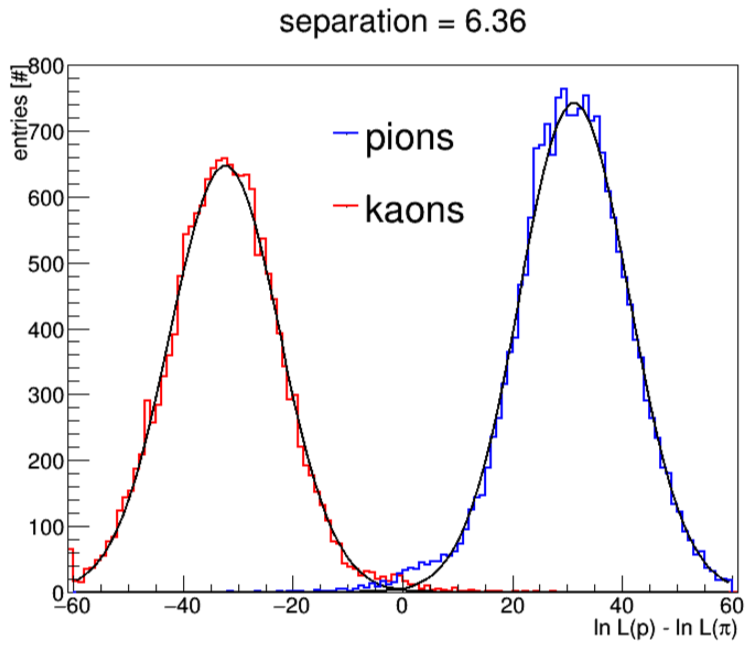
\includegraphics[width=0.43\textwidth]{pics/sepTI300.png} \hspace{0.5cm} 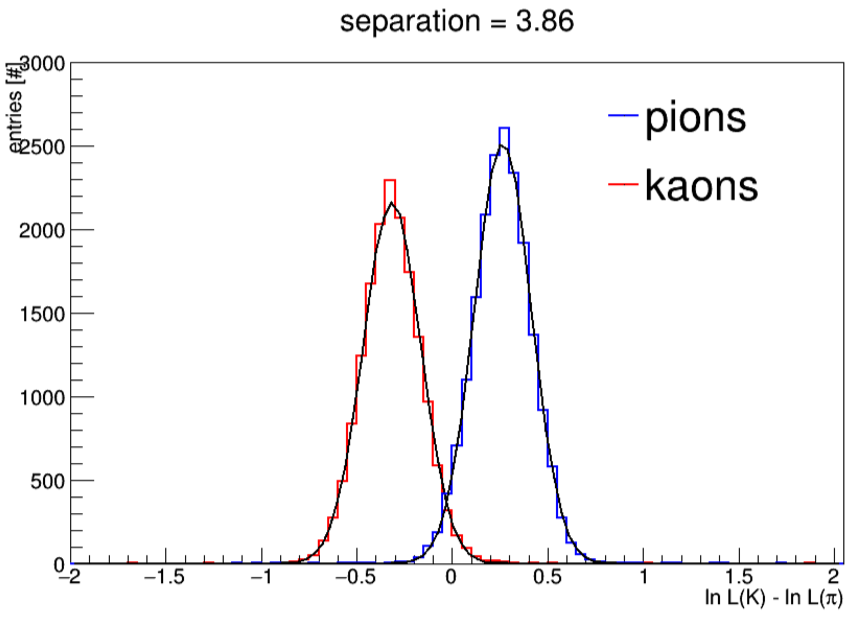
\includegraphics[width=0.52\textwidth]{pics/sepTI1000.png}
\caption{\label{pic:sepTI}
Log likelihoods for kaons (red) and pions (blue) with momenta of $4$ {\gev}/c, and direction defined by $\theta = 4$\mydeg and $\phi = 90$\mydeg. The left plot corresponds to the timing resolution of $300$ ps and it shows 6.4 s.d separation between kaons and pions. The right plot corresponds to $1$ ns timing resolution and it shows 3.9 s.d. separation between kaons and pions. \newline \footnotesize{Different $x$ axis scales are an artefact of the development work: the difference is due to the fact that the log likelihood for the left plot did not have $N$ detected photons in the denominator, and the right plot did have. The number of detected photons for high momentum particles is the same for pions and kaons, therefore this issue does not influence the performance for the given case. }
}
\end{figure}

The separation $S$ between two hypotheses can be calculated based on the difference in log likelihoods (see previous section).

The time imaging reconstruction method is sensitive to the single photon timing resolution. Indeed, the timing information is used here directly, unlike for the geometrical algorithm, where only coarse timing information is needed to cut out some solutions of the reconstructed Cherenkov angle. Figure~\ref{pic:sepTI} shows separation between kaons and pions for two values of the single photon timing resolutions. The single photon timing resolution of 1 ns is approximately the value we are getting experimentally with the PMTs and the electronics boards.
